%-------------------------------------------------------------------------------
%  Theory seminar (30-40 min):
%  "Chiral soliton lattice in inhomogeneous magnetic fields"
%
%  Based on
%    [SS]  D.T. Son, M.A. Stephanov, PRD 77 (2008) 014021 [arXiv:0710.1084]
%    [BY]  T. Brauner, N. Yamamoto, JHEP 04 (2017) 132   [arXiv:1609.05213]
%    [BR]  T. Brauner, R. Radhakrishnan, arXiv:2608.27319
%
%  Compile:  pdflatex csl_seminar  (twice)
%-------------------------------------------------------------------------------
\documentclass[aspectratio=169,10pt]{beamer}

\usetheme[progressbar=frametitle,numbering=fraction,block=fill]{metropolis}
\usepackage{appendixnumberbeamer}
\usepackage[T1]{fontenc}
\usepackage{amsmath,amssymb,bm}
\usepackage{graphicx}
\usepackage{booktabs}
\usepackage{tikz}
\usetikzlibrary{arrows.meta,decorations.pathmorphing}

% ---- colours ------------------------------------------------------------------
\definecolor{myblue}{HTML}{1F4E79}
\definecolor{myred}{HTML}{C0392B}
\definecolor{mygreen}{HTML}{1B7A5A}
\definecolor{myorange}{HTML}{E08214}
\setbeamercolor{frametitle}{bg=myblue}
\setbeamercolor{progress bar}{fg=myorange}
\setbeamercolor{alerted text}{fg=myred}
\setbeamercolor{block title}{bg=myblue!12,fg=myblue}
\setbeamercolor{block body}{bg=myblue!5}

% ---- macros -------------------------------------------------------------------
\newcommand{\B}{\bm{B}}
\newcommand{\Hb}{\bm{H}}
\newcommand{\n}{\bm{n}}
\newcommand{\gr}{\bm{\nabla}}
\newcommand{\fpi}{f_\pi}
\newcommand{\mpi}{m_\pi}
\newcommand{\dd}{\mathrm{d}}
\newcommand{\Bcsl}{B_{\mathrm{CSL}}}
\newcommand{\Bbec}{B_{\mathrm{BEC}}}
\newcommand{\cit}[1]{{\scriptsize\color{gray}[#1]}}
\newcommand{\take}[1]{\begin{block}{}\centering #1\end{block}}

\title{Chiral soliton lattice in inhomogeneous magnetic fields}
\subtitle{What the QCD anomaly does when the magnetic field bends}
\author{R.\ Radhakrishnan}     % <-- edit speaker name / affiliation here
\institute{Department of Physics and Astronomy, North Carolina State University\\[2mm]
  \footnotesize with T.\ Brauner (Stavanger) \quad---\quad \texttt{arXiv:2608.27319}}
\date{Theory seminar}

\begin{document}

\maketitle

%===============================================================================
\begin{frame}{The setting: QCD in a field of $10^{19}$ gauss}
\begin{columns}[T,onlytextwidth]
\begin{column}{0.54\textwidth}
Strong-$B$ QCD is not exotic any more:
\begin{itemize}
  \item magnetar interiors, $B\sim10^{15}$--$10^{19}\,$G;
  \item off-central heavy-ion collisions, the strongest fields ever made;
  \item lattice QCD in a background field.
\end{itemize}
\vspace{2mm}
The interesting scale is set not by $m_\rho^2/e$ but by the \alert{anomaly}:
\[
  \Bcsl=\frac{16\pi \fpi^2\mpi}{\mu}\approx 0.06\,\text{GeV}^2\approx10^{19}\,\text{G}
\]
which \emph{vanishes in the chiral limit}.
\end{column}
\begin{column}{0.44\textwidth}
\begin{block}{The known story (2007--2017)}
Above $\Bcsl$, the QCD ground state at finite $\mu_B$ is not the vacuum and not
nuclear matter: it is a periodic, parity-breaking condensate of \emph{neutral
pions} --- the \alert{chiral soliton lattice}.
\end{block}
\vspace{2mm}
\begin{block}{The fine print}
Every word of that assumes $\B$ is \alert{uniform}. \\[1mm]
In every system we care about, it is not.
\end{block}
\end{column}
\end{columns}
\note{~1 min. Sell the punchline early: the anomaly makes the critical field
parametrically small, and the whole literature assumes uniform B.}
\end{frame}

%===============================================================================
\begin{frame}{The story in four steps}
\begin{enumerate}\setlength{\itemsep}{2.2mm}
  \item[\textbf{I}] \textbf{A wall.} The anomaly gives a $\pi^0$ domain wall a
        baryon number $\propto B$. \cit{Son--Stephanov '07}
  \item[\textbf{II}] \textbf{A lattice.} Solve the EFT exactly: a soliton
        lattice, with an analytic phase diagram. \cit{Brauner--Yamamoto '17}
  \item[\textbf{III}] \textbf{A bent field.} What survives when $\B$ is
        inhomogeneous? \alert{$\leftarrow$ this talk} \cit{TB + RR '26}
  \item[\textbf{IV}] \textbf{What we learned}, and what we still cannot do.
\end{enumerate}
\vspace{4mm}
\begin{block}{The question in one line}
Does the CSL need a uniform magnetic field, or only \emph{some} magnetic field?
\end{block}
\note{~1 min. Say explicitly: I will spend 10 minutes on the known story
because the new results are theorems about it, then 20 on the new work.}
\end{frame}

\section{I. The anomaly builds a wall}

%===============================================================================
\begin{frame}{Why only $\pi^0$ survives}
Two-flavour ChPT, $\Sigma\in SU(2)$, in an external magnetic field:
\[
 \mathcal L=\frac{\fpi^2}{4}\Big[\mathrm{Tr}(D_\nu\Sigma^\dagger D^\nu\Sigma)
 +2\mpi^2\,\mathrm{Re}\,\mathrm{Tr}\,\Sigma\Big]
\]
\begin{itemize}
  \item Charged pions are reorganised into Landau levels,
        $E^2 \supset (2n+1)eB$: for $\sqrt{eB}\gg\mpi$ they are \alert{gapped and
        decouple}.
  \item What is left is a single real field, $\Sigma=e^{i\varphi\tau_3}$ ---
        a \emph{sine-Gordon} theory.
  \item The magnetic field enters that theory only through the
        \alert{Wess--Zumino--Witten} term (the same one that runs
        $\pi^0\to2\gamma$).
\end{itemize}
\vspace{2mm}
\begin{block}{The reduced EFT --- everything below follows from this}
\[
 \mathcal H=\fpi^2\Big[\tfrac12(\gr\varphi)^2+\mpi^2(1-\cos\varphi)
 -\Hb\cdot\gr\varphi\Big],
 \qquad \Hb\equiv\frac{\mu\B}{4\pi^2\fpi^2}
\]
\end{block}
\cit{Son--Zhitnitsky '04; Son--Stephanov '07; Brauner--Yamamoto '17}
\note{~2 min. For a QCD audience this is a reminder, not a derivation.
Stress the power counting: p_CSL = B/(4 pi^2 f^2) must be << 4 pi f.}
\end{frame}

%===============================================================================
\begin{frame}{The anomalous term is a total derivative --- and that is the point}
\begin{columns}[T,onlytextwidth]
\begin{column}{0.52\textwidth}
Since $\gr\cdot\Hb=0$, the term $-\Hb\cdot\gr\varphi$
\begin{itemize}
  \item does \alert{not} enter the equation of motion,
  \item but \alert{does} enter the energy,
  \item and it is \emph{linear} in $\gr\varphi$ --- so it always pays to wind
        $\varphi$ along $\B$.
\end{itemize}
\vspace{2mm}
The anomalous baryon current gives the winding a physical meaning:
\[
  n_B=\frac{\B\cdot\gr\varphi}{4\pi^2},\qquad
  m=\frac{\mu\,\gr\varphi}{4\pi^2}.
\]
\end{column}
\begin{column}{0.48\textwidth}
\begin{block}{Son--Stephanov: the $\pi^0$ domain wall}
$\varphi:0\to2\pi$ across a wall of thickness $1/\mpi$:
\[
 \frac{E}{S}=8\fpi^2\mpi,\qquad \frac{N_B}{S}=\frac{eB}{2\pi}
\]
\[
 \Rightarrow\quad \frac{E}{N_B}=\frac{16\pi \fpi^2\mpi}{eB}
\]
\end{block}
\vspace{1mm}
{\small Beat nuclear matter ($E/N_B\approx m_N$) when
\[
 B>B_1=\frac{16\pi \fpi^2\mpi}{e\,m_N}\approx1.1\times10^{19}\,\mathrm{G}.
\]
Locally stable (no tachyonic $\pi^\pm$ on the wall) above
$B_0=3\mpi^2/e\approx1.0\times10^{19}\,$G.}
\end{column}
\end{columns}
\note{~2.5 min. Key sentence: the wall carries baryon number *because of the
triangle anomaly*, so at finite mu it is a competitive way to store baryons.
Both B_0 and B_1 vanish in the chiral limit -- that is the surprise.}
\end{frame}

%===============================================================================
\begin{frame}{From one wall to a stack}
\begin{columns}[T,onlytextwidth]
\begin{column}{0.5\textwidth}
If one wall is cheaper per baryon than nuclear matter, so are two, so are
$N$\dots\\[2mm]
$\Rightarrow$ the ground state should be a \alert{stack of parallel walls},
their spacing fixed by the competition
\[
 \underbrace{\mpi^2(1-\cos\varphi)}_{\text{likes }\varphi=0}
 \quad\text{vs.}\quad
 \underbrace{-\Hb\cdot\gr\varphi}_{\text{likes winding}}
\]
\end{column}
\begin{column}{0.5\textwidth}
\begin{block}{But a stack is a conjecture}
Son--Stephanov did not solve the EoM for the stack. \\[1.5mm]
Two questions were open:
\begin{itemize}
  \item What \emph{is} the exact ground state?
  \item Where exactly does it appear in the $(\mu,B)$ plane?
\end{itemize}
\end{block}
\end{column}
\end{columns}
\vspace{3mm}
\centering
\alert{That is step II.}
\note{~1 min. This is the hinge of the story: an energetics argument, not a
solution.}
\end{frame}

\section{II. The lattice, solved exactly}

%===============================================================================
\begin{frame}{The pendulum in disguise}
Static, 1D configurations along $\B\parallel\hat z$:
\[
 \partial_z^2\varphi=\mpi^2\sin\varphi
 \qquad\Longleftrightarrow\qquad \text{simple pendulum}
\]
\begin{columns}[T,onlytextwidth]
\begin{column}{0.46\textwidth}
Exact solution in Jacobi elliptic functions,
\[
 \cos\frac{\varphi(z)}{2}=\mathrm{sn}(\bar z,k),\qquad
 \bar z=\frac{z\mpi}{k},
\]
period
\[
 \ell=\frac{2kK(k)}{\mpi}.
\]
\vspace{-1mm}
\begin{itemize}\small
  \item $k\to1$: isolated, widely separated walls
  \item $k\to0$: smooth, almost sinusoidal winding
\end{itemize}
\end{column}
\begin{column}{0.54\textwidth}
\centering
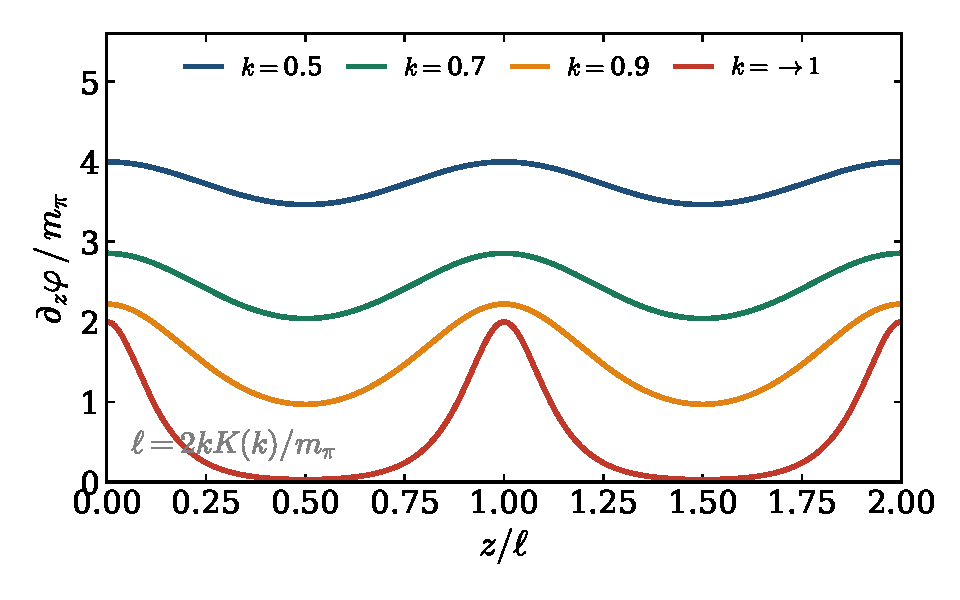
\includegraphics[width=\linewidth]{figs/csl_profile.pdf}\\
{\scriptsize $\partial_z\varphi$ is $\propto$ the baryon density: the lattice
is a periodic array of \emph{topological} objects.}
\end{column}
\end{columns}
\note{~2 min. Emphasise: one integration constant k is left; the ground state
is selected by minimising the *average* energy density, not the EoM.}
\end{frame}

%===============================================================================
\begin{frame}{Selecting the ground state}
\vspace{-1mm}
{\small Average energy density per unit cell:}
\vspace{-2mm}
\[
 \langle\bar{\mathcal E}\rangle
 =4\left[\frac12\Big(1-\frac1{k^2}\Big)+\frac{E(k)}{k^2K(k)}
 -\frac{1}{kK(k)}\frac{\bar H}{\bar H_{\mathrm{CSL}}}\right]
 \ \ \xrightarrow{\ \partial_k=0\ }\ \
 \boxed{\ \frac{E(k)}{k}=\frac{B}{\Bcsl}\ },\quad
 \Bcsl=\frac{16\pi \fpi^2\mpi}{\mu}
\]
\vspace{-3mm}
\begin{center}
{\small Since $E(k)/k\ge1$: \alert{the CSL exists if and only if $B>\Bcsl$}.}\\[1mm]
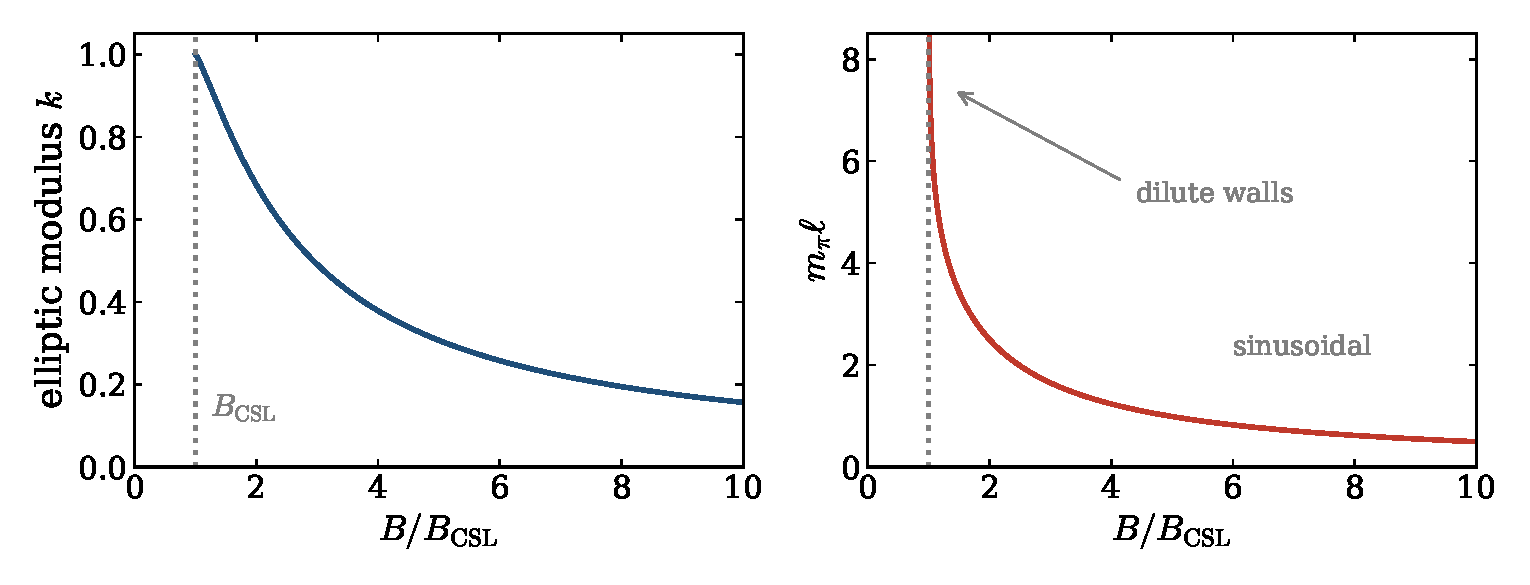
\includegraphics[width=0.78\textwidth]{figs/csl_kofB.pdf}
\end{center}
\note{~2 min. E(k)/k >= 1 is the whole existence proof. Note the transition is
continuous in energy but the period diverges at B_CSL -- infinitely dilute walls.}
\end{frame}

%===============================================================================
\begin{frame}{What makes it a genuine phase}
\begin{columns}[T,onlytextwidth]
\begin{column}{0.5\textwidth}
\textbf{Topological charges per unit cell}
\[
 \frac{N_B}{S}=\frac{B}{2\pi},\qquad \frac{M}{S}=\frac{\mu}{2\pi}
\]
depend only on $\varphi(\pm\ell/2)$, not on the profile.
\vspace{3mm}

\textbf{Broken symmetries}
\begin{itemize}
  \item parity,
  \item continuous translations along $\B$ \\
        $\Rightarrow$ a \alert{phonon} with linear dispersion.
\end{itemize}
\vspace{2mm}
{\small Hierarchical symmetry breaking: chiral symmetry first, then
translations, with $p_{\rm CSL}=B/(4\pi^2\fpi^2)\ll4\pi\fpi$ controlling the
expansion.}
\end{column}
\begin{column}{0.5\textwidth}
\textbf{And an upper edge}: fluctuations of $\pi^\pm$ in the lattice obey a
Lam\'e equation ($n=2$),
\[
 \min\omega^2_{n=0}
 =B-\frac{\mpi^2}{k^2}\Big(2-k^2+2\sqrt{1-k^2+k^4}\Big)
\]
which turns negative at large $B$:
\[
 \Bbec\xrightarrow{\ \mpi\to0\ }\frac{16\pi^4\fpi^4}{\mu^2}
\]
$\Rightarrow$ charged-pion BEC destabilises the CSL from above.
\end{column}
\end{columns}
\note{~2 min. For a QCD audience the Lame operator detail is a one-liner;
the message is that the CSL window is bounded on both sides.}
\end{frame}

%===============================================================================
\begin{frame}{The phase diagram we inherited}
\begin{columns}[T,onlytextwidth]
\begin{column}{0.56\textwidth}
\centering
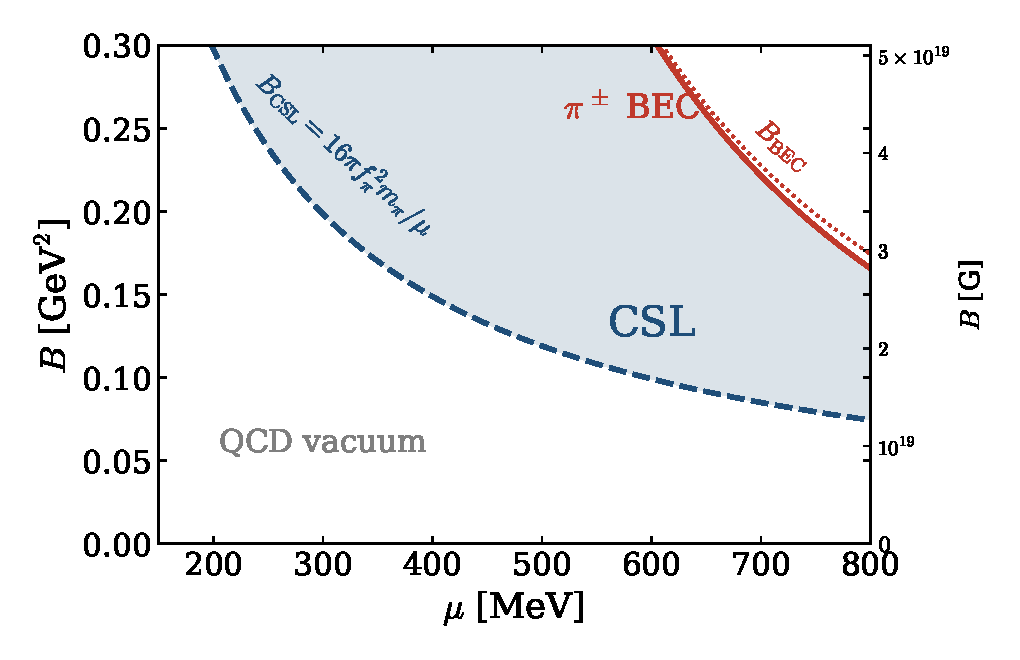
\includegraphics[width=\linewidth]{figs/csl_phase.pdf}
\end{column}
\begin{column}{0.44\textwidth}
\begin{itemize}
  \item Model-independent: leading-order ChPT $+$ anomaly, accurate to
        $p_{\rm CSL}^2/(4\pi \fpi)^2$.
  \item Fully analytic.
  \item Physical window sits right at magnetar field strengths.
\end{itemize}
\vspace{3mm}
\begin{alertblock}{The assumption}
Uniform $\B$, infinite volume.\\[1mm]
Both are wrong in \emph{every} application: heavy-ion fields are violently
inhomogeneous and time-dependent; magnetar fields are dipolar; the lattice is
a finite torus.
\end{alertblock}
\end{column}
\end{columns}
\note{~1.5 min. Curves recomputed from the BY formulae. Land the transition
into the new work here.}
\end{frame}

\section{III. What happens when the field bends}

%===============================================================================
\begin{frame}{Three reasons to care about non-uniform $\B$}
\begin{columns}[T,onlytextwidth]
\begin{column}{0.62\textwidth}
\begin{enumerate}
  \item \textbf{Heavy-ion collisions.} $\B$ varies over the transverse size of
        the fireball and decays on $\sim$fm/$c$ timescales.
  \item \textbf{Compact stars.} Dipolar (or worse) field geometry; the
        variation is slow on QCD scales, but the \emph{geometry} matters ---
        field lines close.
  \item \textbf{Lattice QCD.} On a torus the flux is quantised,
        $eB=2\pi N/(L_xL_y)$. \\[1mm]
        The standard workaround \cit{Levkova--DeTar '14}: make $B$ constant on
        half the lattice and \alert{opposite} on the other half, so the total
        flux vanishes and $B$ can be tuned continuously.\\[1mm]
        $\Rightarrow$ the field \emph{used in simulations} is a magnetic
        domain wall.
\end{enumerate}
\end{column}
\begin{column}{0.38\textwidth}
\begin{block}{Our questions}
\begin{itemize}
  \item Does inhomogeneity destroy the CSL?
  \item If not: for \emph{which} fields does it survive?
  \item Can a bent field ever \emph{help}?
\end{itemize}
\end{block}
\vspace{2mm}
{\small Strategy: same EFT, classical minimisation, but now a finite domain $V$
and a general $\Hb(\bm{x})$.}
\end{column}
\end{columns}
\note{~1.5 min. Point 3 usually wakes up a lattice audience -- the domain-wall
field is not an academic choice, it is what they simulate.}
\end{frame}

%===============================================================================
\begin{frame}{First: a finite box already changes things}
Minimise $\bar E[\varphi]=\int\dd\bar z\,
[\tfrac12(\partial_{\bar z}\varphi)^2+1-\cos\varphi-\bar H\partial_{\bar z}\varphi]$
on $\bar z\in(-\bar L/2,\bar L/2)$, \alert{imposing no boundary condition by hand}.
\begin{columns}[T,onlytextwidth]
\begin{column}{0.48\textwidth}
The variational principle supplies its own:
\[
 \boxed{\ \n\cdot\gr\varphi_0=\n\cdot\Hb\ \ \text{on }\partial V\ }
\]
\begin{itemize}
  \item the ground state is \alert{never} uniform for $\bar H\neq0$;
  \item only a \emph{discrete} set of $k$ is now allowed
        (vs.\ a continuum in infinite volume);
  \item two families: gradient maximal at the centre (I) or minimal (II).
\end{itemize}
\end{column}
\begin{column}{0.52\textwidth}
\centering
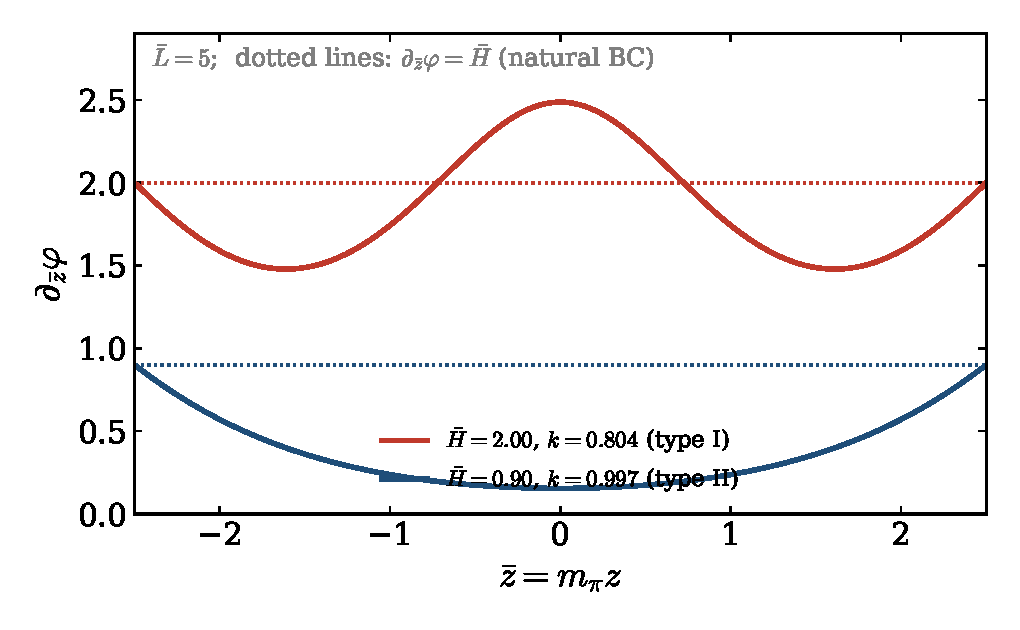
\includegraphics[width=\linewidth]{figs/csl_finitevol.pdf}\\
{\scriptsize Solutions of the EoM satisfying the natural BC at $\bar L=5$.}
\end{column}
\end{columns}
\note{~2 min. The natural (Neumann) BC is the single most important technical
point of the talk -- everything later is built on it.}
\end{frame}

%===============================================================================
\begin{frame}{The finite-volume phase boundary}
\begin{columns}[T,onlytextwidth]
\begin{column}{0.48\textwidth}
\centering
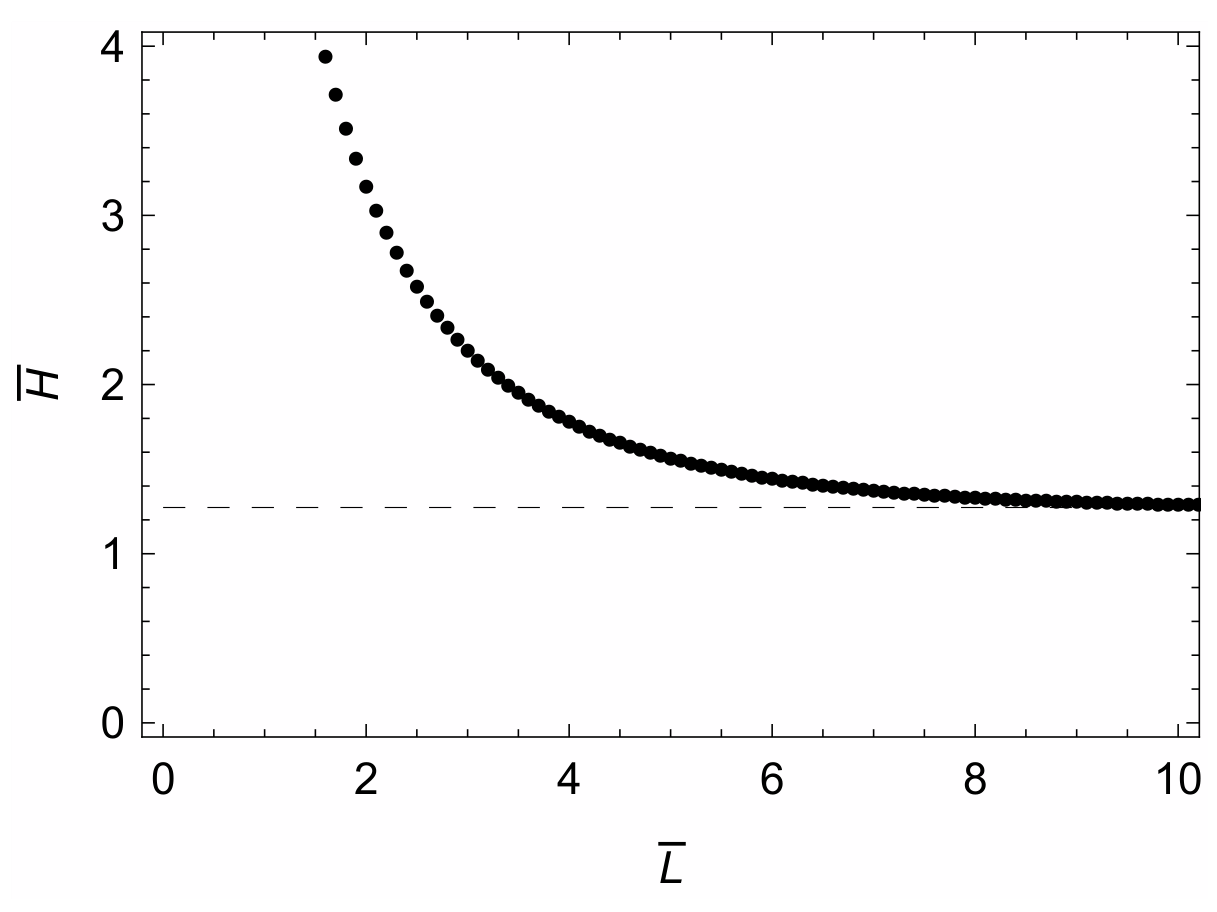
\includegraphics[width=0.96\linewidth]{figs/paper_fig1.png}\\
{\scriptsize Critical field $\bar H_{\rm cr}$ vs.\ box size $\bar L=\mpi L$.
Dashed: infinite-volume value $4/\pi$.}
\end{column}
\begin{column}{0.52\textwidth}
\begin{itemize}
  \item We define the transition as the flip from family II (bending only at
        the boundary) to family I (a soliton in the bulk) --- the
        finite-volume analogue of the domain wall that signals the onset.
  \item $\bar H_{\rm cr}(\bar L)\to4/\pi\approx1.27$, i.e.\ $B\to\Bcsl$,
        as $\bar L\to\infty$. \alert{Good.}
  \item A small box \emph{suppresses} the CSL: you need a stronger field to fit
        a soliton in.
\end{itemize}
\vspace{2mm}
\begin{block}{Why this matters}
Finite-volume corrections are a prerequisite for comparing with lattice QCD ---
and for non-uniform fields, where a thermodynamic limit may not even exist.
\end{block}
\end{column}
\end{columns}
\note{~1.5 min. Also credit T. Kar's master thesis, where finite-volume
effects were first looked at.}
\end{frame}

%===============================================================================
\begin{frame}{The chiral limit: the problem becomes linear}
Set $\mpi=0$. The energy functional
$E[\varphi]=\fpi^2\!\int_V[\tfrac12(\gr\varphi)^2-\Hb\cdot\gr\varphi]$
gives
\[
 \gr^2\varphi_0=0\ \ \text{in }V,
 \qquad \n\cdot\gr\varphi_0=\n\cdot\Hb\ \ \text{on }\partial V.
\]
\vspace{-2mm}
\begin{block}{A Neumann problem for the Laplace equation}
Solution exists and is \alert{unique up to a constant shift} --- so in the
chiral limit there is exactly one stationary state, and it is automatically the
ground state. No competition, no phase transition.
\end{block}
\vspace{2mm}
The whole question ``which fields support a CSL?'' is now the question:
\begin{center}
\emph{what does the map $\ \Hb\ \longmapsto\ \varphi_0[\Hb]\ $ look like?}
\end{center}
\note{~1.5 min. Selling point: in the chiral limit the sine-Gordon problem
collapses to electrostatics, and we can be *complete*, not illustrative.}
\end{frame}

%===============================================================================
\begin{frame}{The answer: $\varphi_0$ is the magnetic scalar potential}
Decompose the field on the domain $V$ (gradient--solenoid / Helmholtz):
\[
 \Hb=\gr\psi[\Hb]+\bm{A}[\Hb],\qquad
 \gr\cdot\bm{A}=0\ \text{in }V,\quad \n\cdot\bm{A}=0\ \text{on }\partial V.
\]
Complete the square in the energy:
\[
 E[\varphi]=\fpi^2\!\int_V\Big[\tfrac12(\gr\varphi-\gr\psi)^2-\tfrac12(\gr\psi)^2
 \underbrace{-\bm{A}\cdot\gr\varphi}_{\text{integrates to }0}\Big]
\]
\[
 \Longrightarrow\quad
 \boxed{\ E[\varphi]\ \ge\ -\frac{\fpi^2}{2}\int_V(\gr\psi)^2\ \ge\
 -\frac{\fpi^2}{2}\int_V \Hb^2\ }
\]
\begin{itemize}
  \item first bound saturated $\iff\gr\varphi=\gr\psi$: \alert{the ground state
        is $\psi[\Hb]$};
  \item second bound saturated $\iff\bm{A}=0$, i.e.\ $\Hb$ is
        \alert{conservative}.
\end{itemize}
\note{~2.5 min. This slide is the theoretical core. Do the algebra out loud:
the A term drops because it is divergence-free inside and tangential on the
boundary.}
\end{frame}

%===============================================================================
\begin{frame}{Two theorems, and a picture}
\vspace{-2mm}
\begin{center}
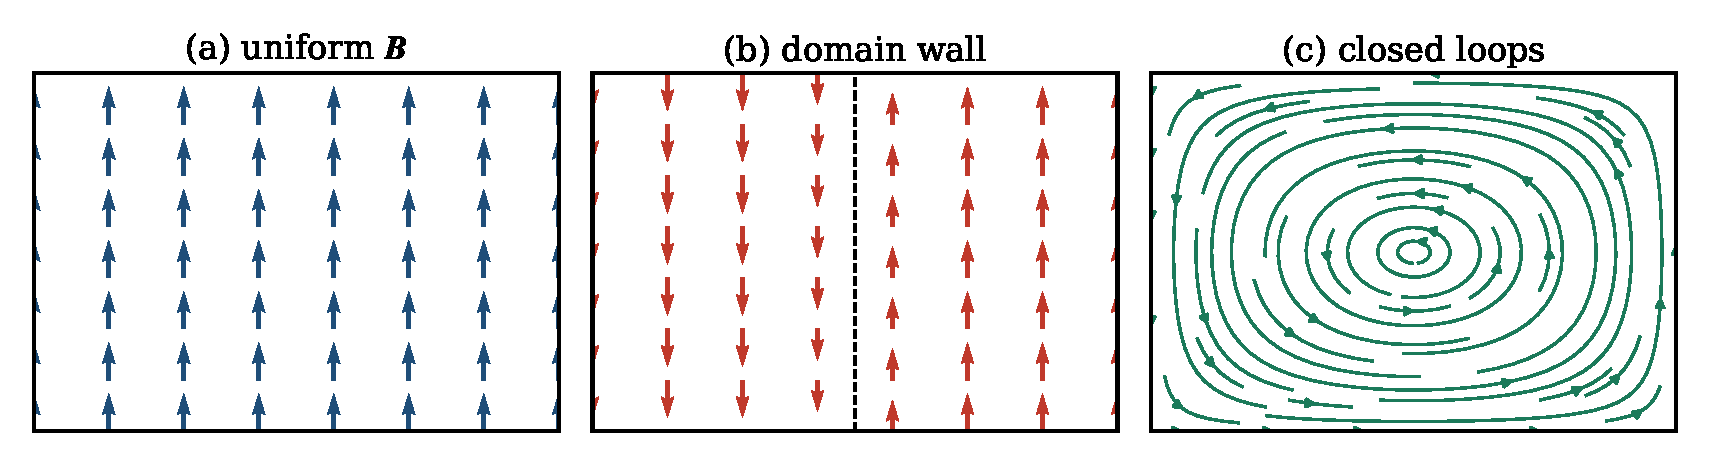
\includegraphics[width=0.92\textwidth]{figs/csl_geometries.pdf}
\end{center}
\vspace{-3mm}
\begin{columns}[T,onlytextwidth]
\begin{column}{0.48\textwidth}
\begin{block}{1. When is there \emph{no} CSL?}
{\small $E\le0$ always, with equality iff $\gr\psi=0$ --- exactly when $\B$ is
\alert{tangential to $\partial V$ everywhere} \textbf{(c)}. Any field that pokes
through the boundary condenses pions.}
\end{block}
\end{column}
\begin{column}{0.48\textwidth}
\begin{block}{2. When is the CSL \emph{optimal}?}
{\small The bound $-\tfrac{\fpi^2}{2}\!\int\!\Hb^2$ is reached iff $\Hb$ is
conservative \textbf{(a)}. Then $\gr\varphi_0=\Hb$ \emph{pointwise}: the gradient
\alert{follows the field lines}, whatever the shape of $V$.}
\end{block}
\end{column}
\end{columns}
\vspace{1mm}
\centering
{\small For non-conservative fields \textbf{(b)}, both the decomposition and
$\varphi_0$ depend on the domain --- \emph{boundaries are physical}.}
\note{~2 min. Punchline to say out loud: inhomogeneity per se is not the enemy;
*closed field lines* are.}
\end{frame}

%===============================================================================
\begin{frame}{A worked family: separation of variables}
Take $\Hb(x,z)=(0,H(x))$ on a rectangle $|x|\le L_x/2$, $|z|\le L_z/2$:
{\small
\[
 \varphi_0(x,z)=\frac{z}{L_x}\!\int\! \dd t\,H(t)
 +\!\!\sum_{\text{even }n>0}\!\!\frac{2\!\int\!\dd t\,H(t)\cos\frac{\pi nt}{L_x}}
 {\pi n\cosh\frac{\pi nL_z}{2L_x}}\cos\frac{\pi nx}{L_x}\sinh\frac{\pi nz}{L_x}
 +\!\!\sum_{\text{odd }n>0}\!\!(\cos\leftrightarrow\sin)
\]}
\vspace{-3mm}
\begin{columns}[T,onlytextwidth]
\begin{column}{0.5\textwidth}
For the \alert{magnetic domain wall} $H_{\rm DW}=H_0\,\mathrm{sgn}\,x$ only the
odd sum survives:
\[
 \varphi_{\rm DW}=\!\!\sum_{\text{odd }n>0}\!\!
 \frac{4H_0L_x}{\pi^2n^2\cosh\frac{\pi nL_z}{2L_x}}
 \sin\frac{\pi nx}{L_x}\sinh\frac{\pi nz}{L_x}
\]
\end{column}
\begin{column}{0.5\textwidth}
and as $L_x\to\infty$ the sum becomes an integral,
\[
 \varphi_{\rm DW}\to\frac{H_0}{\pi}\int_{-\infty}^{+\infty}\!\!\dd k\,
 \frac{\sin kx\,\sinh kz}{k^2\cosh\frac{kL_z}{2}}.
\]
\vspace{1mm}
{\small These closed forms are what we use to benchmark the numerics later.}
\end{column}
\end{columns}
\note{~1 min. Do not read the formula; say "it is electrostatics on a
rectangle" and move on. It matters because it gives exact benchmarks.}
\end{frame}

%===============================================================================
\begin{frame}{Bonus: a non-uniform chemical potential comes for free}
If $\mu=\mu(\bm x)$ (local equilibrium in an inhomogeneous system), then
$\Hb=\mu\B/(4\pi^2\fpi^2)$ is no longer solenoidal and
\[
 \gr^2\varphi_0=\gr\cdot\Hb=\frac{\B\cdot\gr\mu}{4\pi^2\fpi^2},
\]
a \emph{Poisson} equation --- with the same natural BC.
\vspace{2mm}
\begin{itemize}
  \item The decomposition $\Hb=\gr\psi+\bm A$ still holds ($\bm A$ is still
        divergence-free and tangential), so $\varphi_0=\psi[\Hb]$ \alert{still}.
  \item Neither bound used $\gr\cdot\Hb=0$: every statement survives verbatim,
        phrased in terms of $\Hb$ rather than $\B$.
  \item CSL still beats the vacuum unless $\B$ is tangential to $\partial V$
        --- \emph{independently of $\mu(\bm x)$}.
  \item The optimal bound now requires $\Hb$ conservative:
        $\ \gr\mu\times\B+\mu\,\gr\times\B=\bm0$.
\end{itemize}
\note{~1 min. Cheap generalisation, but it is the one relevant for a realistic
star or fireball. Flag it as a by-product.}
\end{frame}

%===============================================================================
\begin{frame}{Massive pions: back to non-linearity, but two facts survive}
Now $\mpi\neq0$ and the EoM is non-linear again. Still, without any computation:
\vspace{1mm}
\begin{block}{Fact 1 --- a no-go}
The mass term is non-negative, so $E\ge E|_{\mpi=0}\ge0$ for fields tangential
to $\partial V$. \alert{Tangential fields never produce a CSL, at any $\mpi$.}
\end{block}
\begin{block}{Fact 2 --- a guarantee}
Use $\psi[\Hb]$ as a variational trial state:
\[
 E[\psi]=\fpi^2\!\int_V\Big[-\tfrac12(\gr\psi)^2+\mpi^2(1-\cos\psi)\Big]
\]
For conservative fields $\gr\psi=\Hb$, and the integrand is negative everywhere
provided $|\Hb|>2\mpi$, i.e.
\[
 \boxed{\ |\B|>\frac{8\pi^2\fpi^2\mpi}{\mu}=\frac{\pi}{2}\Bcsl\approx0.09\ \text{GeV}^2\ }
\]
\centering \alert{Remarkably close to the uniform-field threshold} --- and valid
for \emph{any} domain $V$.
\end{block}
\note{~2 min. Emphasise the logic: Fact 2 is a variational bound, so it is a
sufficient condition for CSL, not a phase boundary. That is why it can sit
above the Fig. 1 curve without contradiction.}
\end{frame}

%===============================================================================
\begin{frame}{Numerics: what we do, and why you should believe it}
\begin{columns}[T,onlytextwidth]
\begin{column}{0.52\textwidth}
\textbf{Method} (\textsc{Mathematica} 15, built from scratch)
\begin{itemize}\small
  \item discretise $V$ on an $n_x\times n_z$ grid;
  \item central differences in the bulk, one-sided at the edge;
  \item trapezoidal rule (higher-order integrators develop artifacts on
        modulated states);
  \item minimise over \emph{all} grid values --- \alert{no boundary condition
        imposed}, the natural BC emerges;
  \item \texttt{NMinimize} (global, coarse) cross-checking
        \texttt{FindMinimum} (local, fine).
\end{itemize}
\vspace{1mm}
\textbf{Validation}: scan $0<\bar L\le10$, $0<\bar H\le5$ on a $50\times50$
grid: the code finds the true global minimum at \alert{2495 of 2500} points
(the five misses sit on curves of degenerate minima).
\end{column}
\begin{column}{0.48\textwidth}
\centering
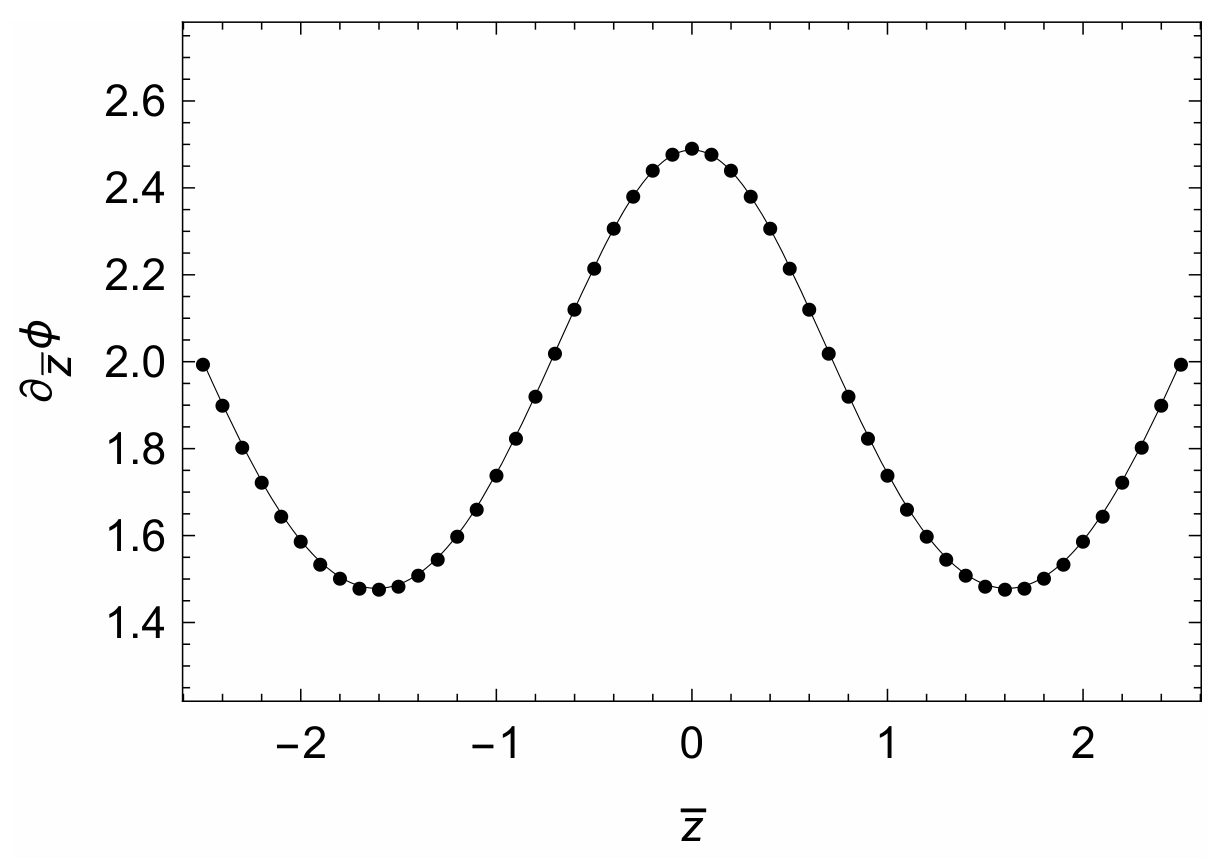
\includegraphics[width=0.95\linewidth]{figs/paper_fig2.png}\\
{\scriptsize 1D benchmark, $\bar L=5,\bar H=2$: points = free minimisation on
50 cells, line = analytic solution. Note $\partial_{\bar z}\varphi=\bar H=2$
at the edges --- the natural BC, found, not imposed.}
\end{column}
\end{columns}
\note{~2 min. A QCD audience will ask about the continuum limit -- pre-empt it:
discretisation artifacts are small as long as the cell is smaller than the pion
Compton wavelength, n >~ m_pi L. Backup slide has the numbers.}
\end{frame}

%===============================================================================
\begin{frame}{Two dimensions: a Gaussian blob of field}
\begin{columns}[T,onlytextwidth]
\begin{column}{0.44\textwidth}
\centering
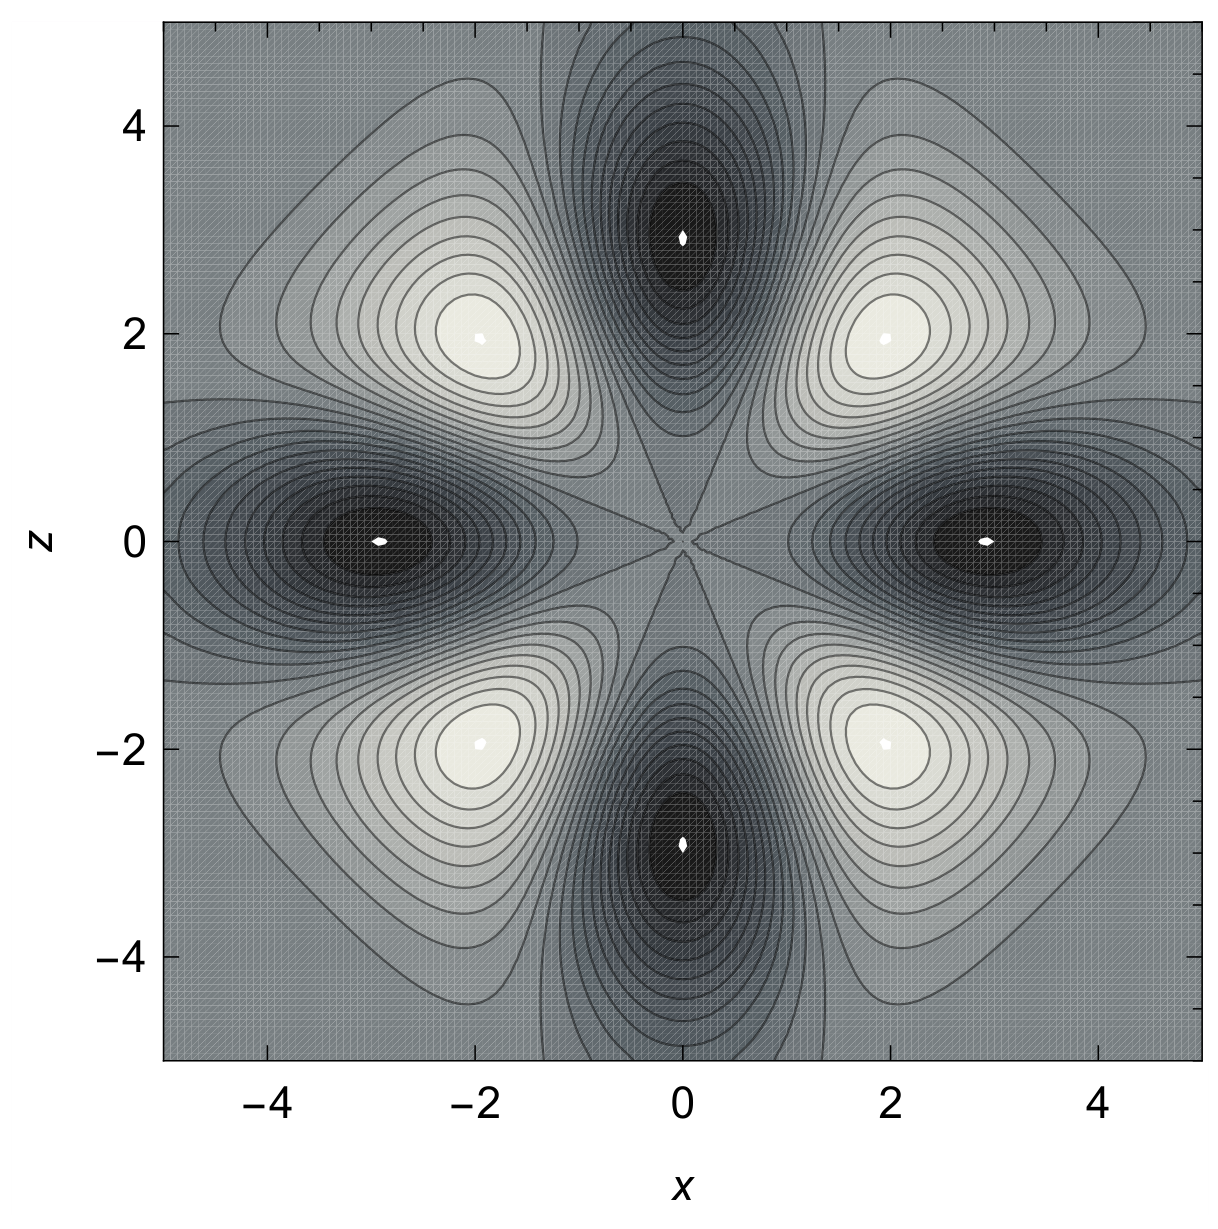
\includegraphics[width=0.93\linewidth]{figs/paper_fig3.png}
\end{column}
\begin{column}{0.56\textwidth}
Field from a Gaussian scalar potential,
$\psi=\psi_0e^{-(x^2+z^2)/R^2}$, $\Hb=(-\partial_z\psi,\partial_x\psi)$,
in the chiral limit on a $10\times10$ box.
\vspace{2mm}
\begin{itemize}
  \item Plotted: the anomalous baryon density $\Hb\cdot\gr\varphi$.
  \item Bright lobes = positive baryon density, dark = negative.
  \item The condensate \emph{textures itself} to the field: the lattice is no
        longer a stack of flat planes, it is a curved, locally-defined object.
\end{itemize}
\vspace{2mm}
{\small This is an honest 2D minimisation on a $51\times51$ grid --- no ansatz.}
\end{column}
\end{columns}
\note{~1.5 min. Good slide to slow down on: it is the first *picture* of a CSL
in a bent field.}
\end{frame}

%===============================================================================
\begin{frame}{The case study: a magnetic domain wall}
\begin{columns}[T,onlytextwidth]
\begin{column}{0.44\textwidth}
\centering
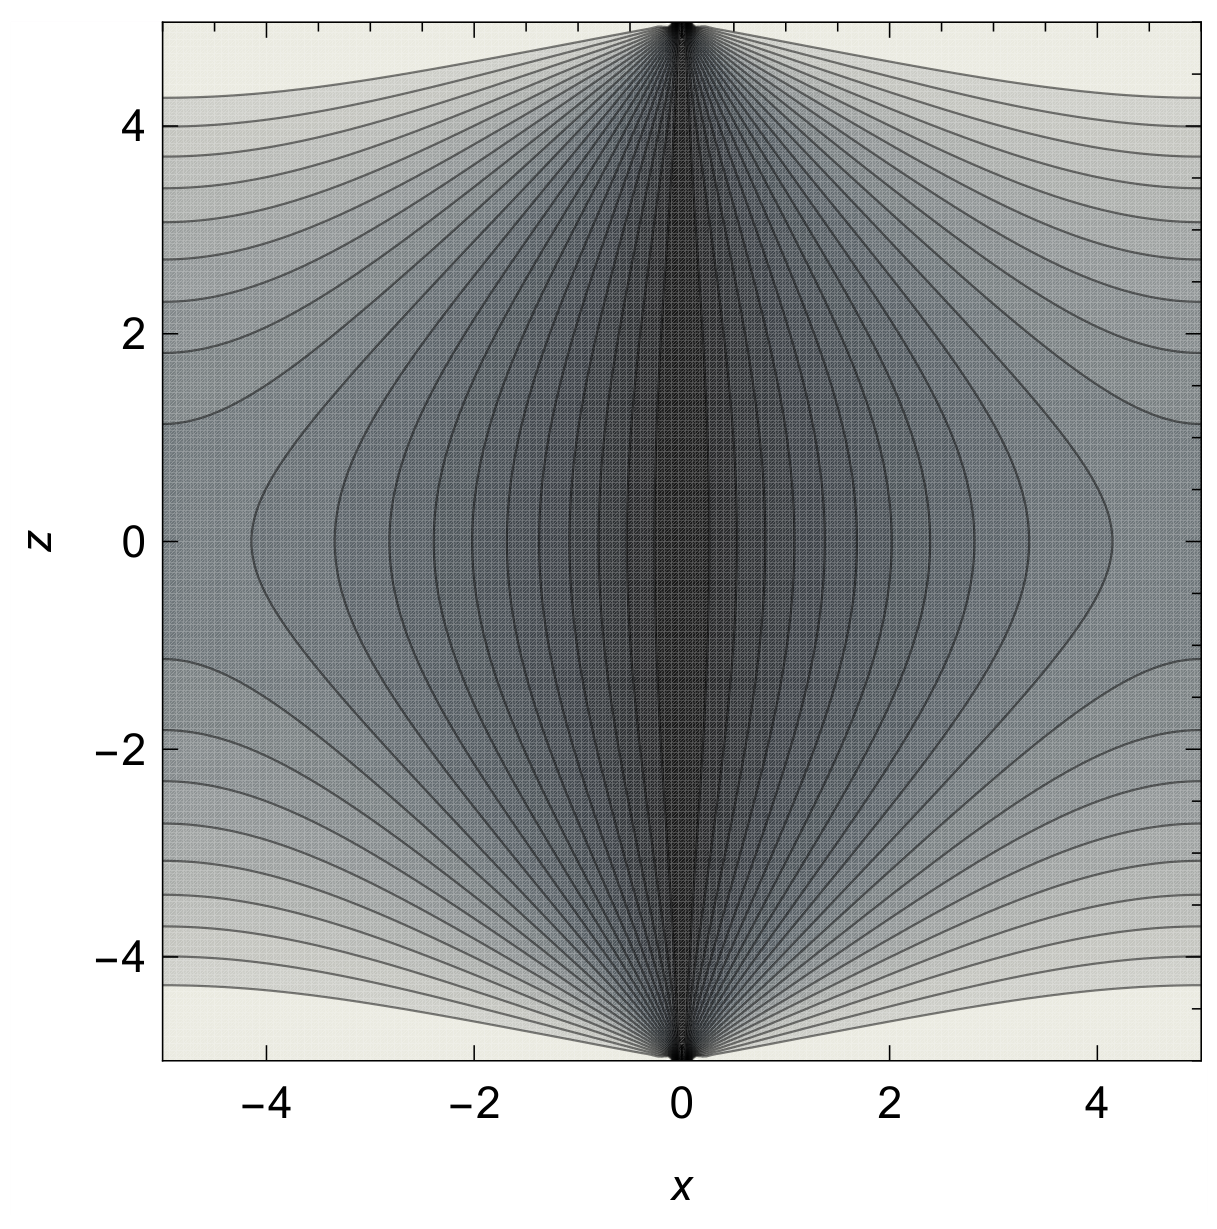
\includegraphics[width=0.93\linewidth]{figs/paper_fig4.png}
\end{column}
\begin{column}{0.56\textwidth}
$H_\xi(x)=H_0\tanh(x/\xi)$: constant field of opposite sign on the two halves
--- exactly the lattice-QCD trick.
\vspace{2mm}
\begin{itemize}
  \item The CSL \alert{survives}, even though this field is \emph{not}
        conservative.
  \item Baryon density vanishes on the wall at $x=0$ and is symmetric about it.
  \item $\xi$ interpolates between a sharp wall ($\xi\to0$) and a field
        effectively linear in $x$ ($\xi\gtrsim L_x$).
\end{itemize}
\vspace{2mm}
\begin{block}{Benchmark}
Chiral limit, square domain, sharp wall: analytics predict
$\langle\mathcal E_{\rm DW}\rangle=\mathcal E_0/2$ exactly;
the code gives $0.499\,\mathcal E_0$ on a $31\times31$ grid, independently of $L$.
\end{block}
\end{column}
\end{columns}
\note{~2 min. "Not conservative, and yet fine" is the sentence that answers the
title question for the lattice community.}
\end{frame}

%===============================================================================
\begin{frame}{How much does bending cost?}
\begin{columns}[T,onlytextwidth]
\begin{column}{0.5\textwidth}
\centering
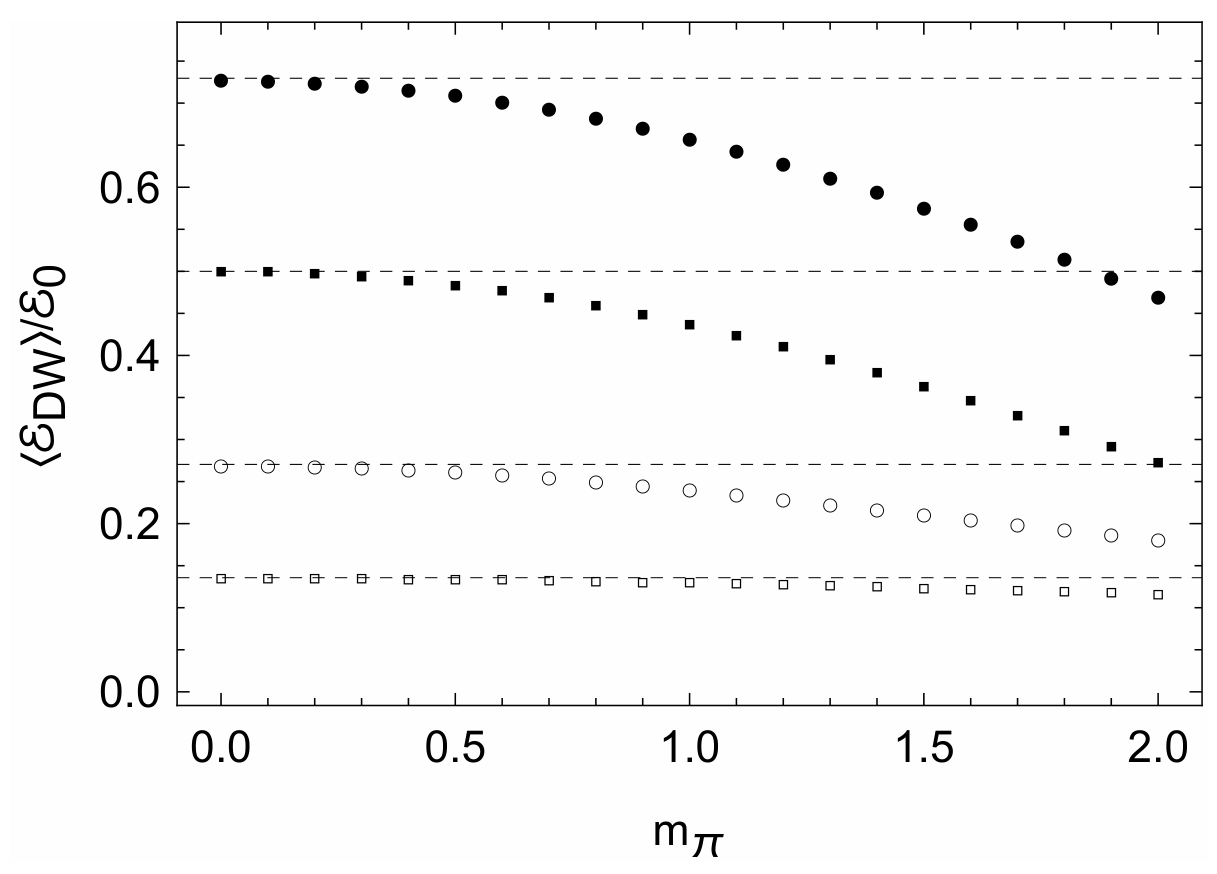
\includegraphics[width=0.86\linewidth]{figs/paper_fig5.png}\\
{\scriptsize Energy vs.\ pion mass, for aspect ratios
$\alpha=L_z/L_x=0.5,1,2,4$ (sharp wall, $H_0=5$).}
\end{column}
\begin{column}{0.5\textwidth}
\centering
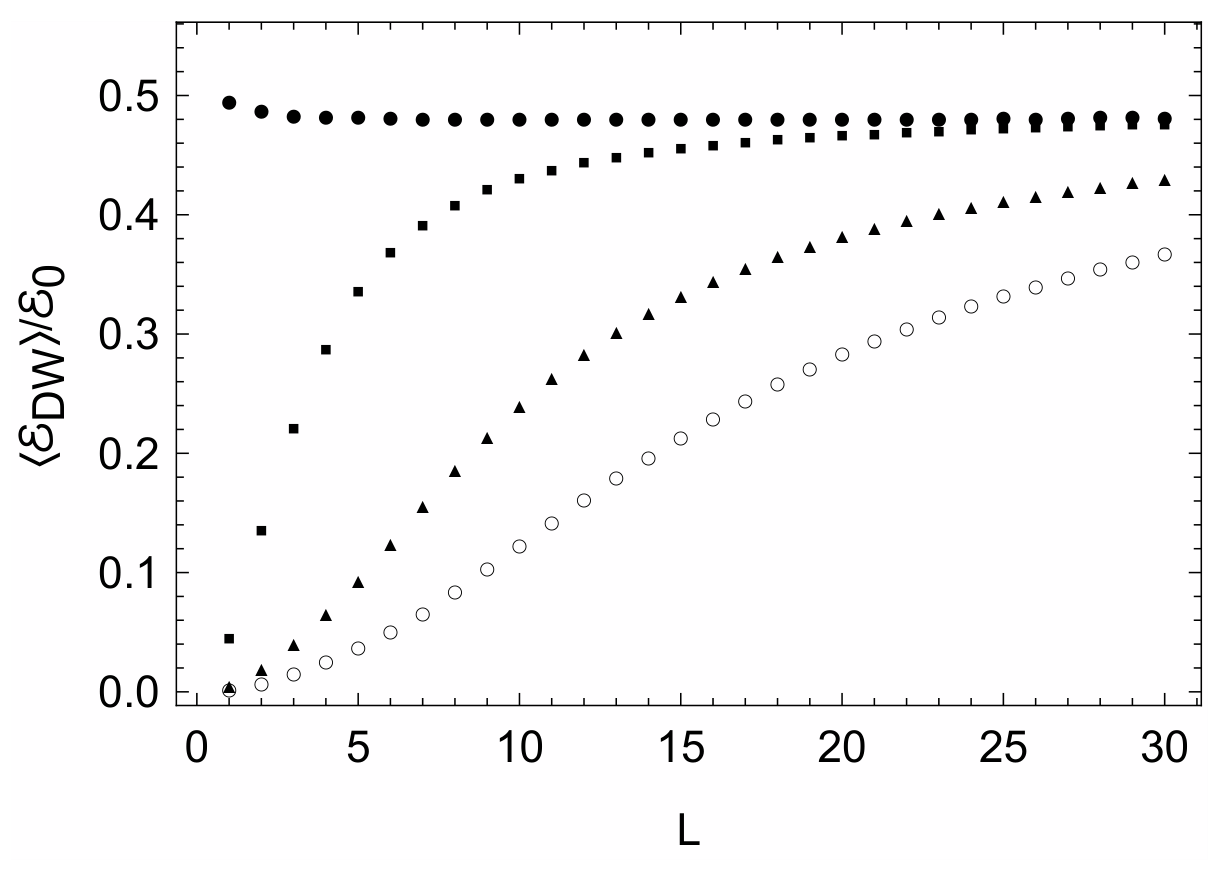
\includegraphics[width=0.86\linewidth]{figs/paper_fig6.png}\\
{\scriptsize Energy vs.\ system size, for wall widths
$\xi\to0,1,3,5$ ($\mpi=0.5$).}
\end{column}
\end{columns}
\vspace{1mm}
{\small
\begin{itemize}\setlength{\itemsep}{0.4mm}
  \item $\mpi\to0$ intercepts reproduce the analytic values (dashed) --- the
        code is right.
  \item Increasing $\mpi$ monotonically \emph{reduces} the condensation energy:
        the mass term fights the winding.
  \item Condensation switches off for $L\lesssim\xi$ and saturates for $L\gg\xi$.
\end{itemize}}
\note{~1.5 min. The qualitative statement: bending typically costs you
condensation energy, but never all of it.}
\end{frame}

%===============================================================================
\begin{frame}{The analytic gem: how much energy lives \emph{on} the wall?}
In the chiral limit the domain-wall energy can be summed in closed form:
\[
 \frac{\langle\mathcal E_{\rm DW}\rangle}{\mathcal E_0}
 =\frac{16}{\alpha}\sum_{\text{odd }n>0}\frac{1}{(\pi n)^3}
 \tanh\frac{\pi n\alpha}{2},\qquad \alpha=\frac{L_z}{L_x}
\]
Using the \alert{fermionic Matsubara identity}
$\sum_{\text{odd }k>0}(k^2+t^2)^{-1}=\frac{\pi}{4t}\tanh\frac{\pi t}{2}$:
\begin{columns}[T,onlytextwidth]
\begin{column}{0.52\textwidth}
\[
 \frac{\langle\mathcal E_{\rm DW}\rangle}{\mathcal E_0}
 =1-\frac{14\alpha\zeta(3)}{\pi^3}
 +\frac{32\alpha}{\pi^3}\!\!\sum_{\text{odd }k>0}\!\frac{1}{k^3}
 \frac{1}{e^{\pi k/\alpha}+1}
\]
\begin{itemize}\small
  \item the first two terms are the \emph{entire} power series in $\alpha$;
  \item everything else is exponentially small;
  \item $\alpha\to0$: the uniform-field answer, $\mathcal E_0$;
  \item $\alpha=1$: exactly $\mathcal E_0/2$.
\end{itemize}
\end{column}
\begin{column}{0.48\textwidth}
\centering
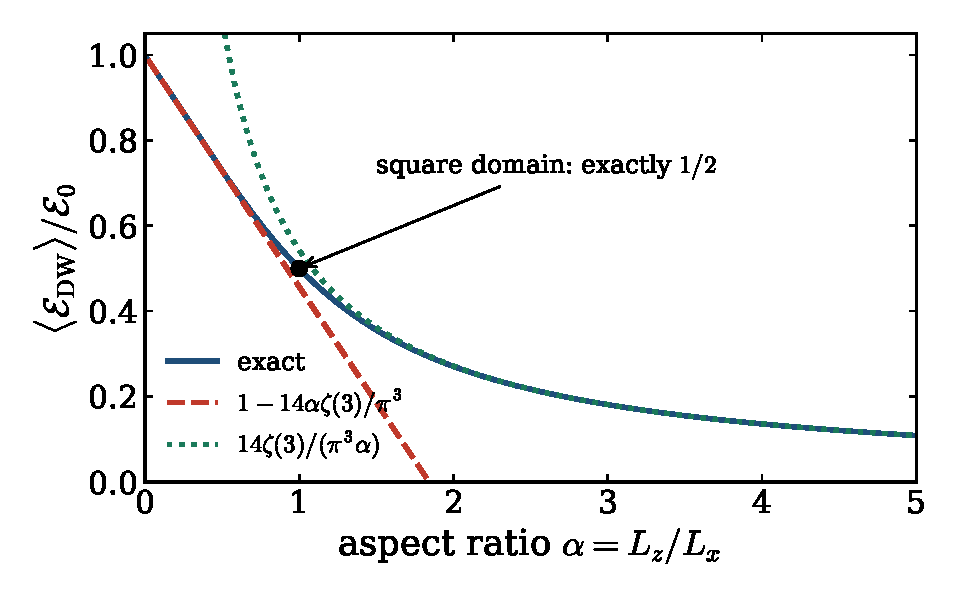
\includegraphics[width=\linewidth]{figs/csl_dwenergy.pdf}
\end{column}
\end{columns}
\vspace{-1mm}
\centering
{\small Linear in $\alpha$ $\Rightarrow$ energy excess $\propto L_x^0L_z^2$:
\alert{localised on the wall}.}
\note{~2 min. This is the slide to be proud of: a Matsubara sum showing up in
a magnetostatics problem, and it tells you the energy cost is a surface term.}
\end{frame}

\section{IV. Where this leaves us}

%===============================================================================
\begin{frame}{Summary}
\begin{block}{1. Inhomogeneity does not kill the CSL --- geometry decides}
$\B$ tangential to the boundary everywhere $\Rightarrow$ no condensation, at
any pion mass. Anything else $\Rightarrow$ the vacuum is unstable.
\end{block}
\begin{block}{2. Conservative fields are the friendly case}
Chiral limit: $\gr\varphi_0=\Hb$ pointwise, the energy saturates its bound and
does not care about the domain. Massive: a CSL is \emph{guaranteed} for
$|\B|>\tfrac{\pi}{2}\Bcsl\approx0.09\,$GeV$^2$, for any $V$.
\end{block}
\begin{block}{3. Bending costs, but not much, and it is a surface effect}
For the lattice-QCD domain-wall field, the cost is exactly computable in the
chiral limit and localised on the wall:
$\langle\mathcal E_{\rm DW}\rangle/\mathcal E_0=1-14\alpha\zeta(3)/\pi^3+\dots$
\end{block}
\vspace{1mm}
\centering
{\small Along the way: the finite-volume CSL phase boundary, and a working
2D energy minimiser with no boundary conditions imposed by hand.}
\note{~1.5 min.}
\end{frame}

%===============================================================================
\begin{frame}{What we cannot do yet}
\begin{columns}[T,onlytextwidth]
\begin{column}{0.47\textwidth}
\textbf{Excitations.}
The ground state is one property; transport and thermodynamics need the
spectrum. In a uniform field it is a Lam\'e problem. In a bent field, the
phonon is no longer a plane wave --- and it is not even obvious what the
Nambu--Goldstone counting is.
\vspace{3mm}

\textbf{Realistic fields.}
We used mathematically clean profiles. A dipole field, or an event-by-event
heavy-ion field, is the honest next step --- and would turn this into a
phenomenological statement.
\end{column}
\hfill
\begin{column}{0.47\textwidth}
\textbf{Beyond the classical minimisation.}
Thermal and quantum fluctuations shift the phase boundary already in the
uniform case \cit{Brauner--Kole\v{s}ov\'a--Yamamoto '21; NLO '23}. With
inhomogeneity, that computation is open.
\vspace{3mm}

\textbf{And a different attack.}
The sine-Gordon-plus-anomaly Hamiltonian discretises cleanly onto a qubit
register (clock/shift operators, $\Pi^2$ from the QFT). The magnetic term
needs $\ge2$ qubits per site to be non-trivial --- first steps towards
simulating the real-time formation of a CSL. \emph{(backup)}
\end{column}
\end{columns}
\note{~1.5 min. End on questions you want the audience to ask.}
\end{frame}

%===============================================================================
\begin{frame}[standout]
Thank you\\[4mm]
{\normalsize\rmfamily
Bending the magnetic field costs condensation energy,\\
but only closing the field lines destroys the lattice.}
\end{frame}

%===============================================================================
\appendix

\begin{frame}{Backup: finite-volume energies}
With $\theta=\varphi-\pi$, $\theta=2\,\mathrm{am}\big(\frac{\bar z-\bar z_0}{k},k\big)$,
the energy on $\bar z\in(-\bar L/2,\bar L/2)$ is
\[
 \bar E(k,\bar z_0)=2\bar L\Big(1-\frac1{k^2}\Big)
 +\frac4k\Big[\mathcal E\big(\tfrac{\bar z-\bar z_0}{k},k\big)\Big]_{-\bar L/2}^{+\bar L/2}
 -2\bar H\Big[\mathrm{am}\big(\tfrac{\bar z-\bar z_0}{k},k\big)\Big]_{-\bar L/2}^{+\bar L/2}
\]
\textbf{Family I} ($\bar z_0=0$, gradient maximal at the centre):
\[
 \bar E_{\max}(k)=2\bar L\Big(1-\frac1{k^2}\Big)+\frac8k\mathcal E\big(\tfrac{\bar L}{2k},k\big)
 -4\bar H\,\mathrm{am}\big(\tfrac{\bar L}{2k},k\big)
\]
\textbf{Family II} ($\bar z_0=kK(k)$, gradient minimal at the centre):
\[
 \bar E_{\min}(k)=2\bar L\Big(1-\frac1{k^2}\Big)+\frac8k\mathcal E\big(\tfrac{\bar L}{2k},k\big)
 -8k\,\mathrm{sn}\,\mathrm{cd}\big(\tfrac{\bar L}{2k},k\big)
 -2\bar H\Big[\mathrm{am}\big(\tfrac{\bar L}{2k}+K,k\big)+\mathrm{am}\big(\tfrac{\bar L}{2k}-K,k\big)\Big]
\]
$\mathcal E$ = Jacobi epsilon function. The natural BC selects a discrete set of
$k$; the ground state is the one of lowest $\bar E$.
\end{frame}

\begin{frame}{Backup: charged pions in the lattice}
Fluctuation equation for $\pi^+$ in the CSL background:
\[
 \big[-\partial_z^2+6k^2\mathrm{sn}^2(\bar z,k)\big]\tilde\pi_+
 =\frac{k^2}{\mpi^2}\big[\omega^2-(2n+1)B\big]\tilde\pi_++(k^2+4)\tilde\pi_+
\]
a Lam\'e operator with $n=2$ $\Rightarrow$ three bands; the lowest band edge gives
\[
 \min\omega^2_{n=0}=B-\frac{\mpi^2}{k^2}\big(2-k^2+2\sqrt{1-k^2+k^4}\big).
\]
\begin{itemize}
  \item At $k\to1$ (single wall) this is $B-3\mpi^2$: Son--Stephanov's $B_0$.
  \item At large $B$, $k\propto1/B$, so the second term $\sim B^2$: BEC always
        wins eventually.
  \item Chiral limit: $\Bbec=16\pi^4\fpi^4/\mu^2$.
\end{itemize}
\end{frame}

\begin{frame}{Backup: discretisation control}
The EFT has one intrinsic scale, the pion Compton wavelength $1/\mpi$.
A cell of size $L_x/(n_x-1)\times L_z/(n_z-1)$ is safe when
\[
 n_x\gtrsim\mpi L_x,\qquad n_z\gtrsim\mpi L_z.
\]
\textbf{Example.} Uniform field, $H_0=5$, $\mpi=0.5$, $L=20$, $31\times31$ grid:
\[
 \langle\mathcal E\rangle_{\rm num}=-12.36
 \quad\text{vs.}\quad
 \langle\mathcal E\rangle_{\rm exact}=-12.25
 \qquad(\sim1\%).
\]
\vspace{1mm}
The sharp-domain-wall benchmark in the chiral limit gives $0.499\,\mathcal E_0$
against the exact $0.5\,\mathcal E_0$ ($0.2\%$ on a $31\times31$ grid), improving
with refinement.
\vspace{2mm}
\begin{block}{Caveat we state in the paper}
Do not vary $\mpi$, $L$, $\xi$ at fixed grid size without rechecking these
inequalities --- the continuum limit is expensive because the number of
optimisation variables grows as $n_xn_z$.
\end{block}
\end{frame}

\begin{frame}{Backup: the wide-domain limit}
From the exact representation,
\[
 \frac{\langle\mathcal E_{\rm DW}\rangle}{\mathcal E_0}
 \xrightarrow{\ \alpha\to\infty\ }\frac{14\zeta(3)}{\pi^3\alpha},
\]
so the total energy scales as $L_x^2L_z^0$ --- in the opposite (thin-slab) limit
$\alpha\to0$ the deficit scales as $L_x^0L_z^2$.
\vspace{2mm}

Physically: for a tall thin box the wall dominates the whole sample; for a wide
flat box the wall is a negligible perturbation on a uniform-field CSL.
\vspace{4mm}

\centering
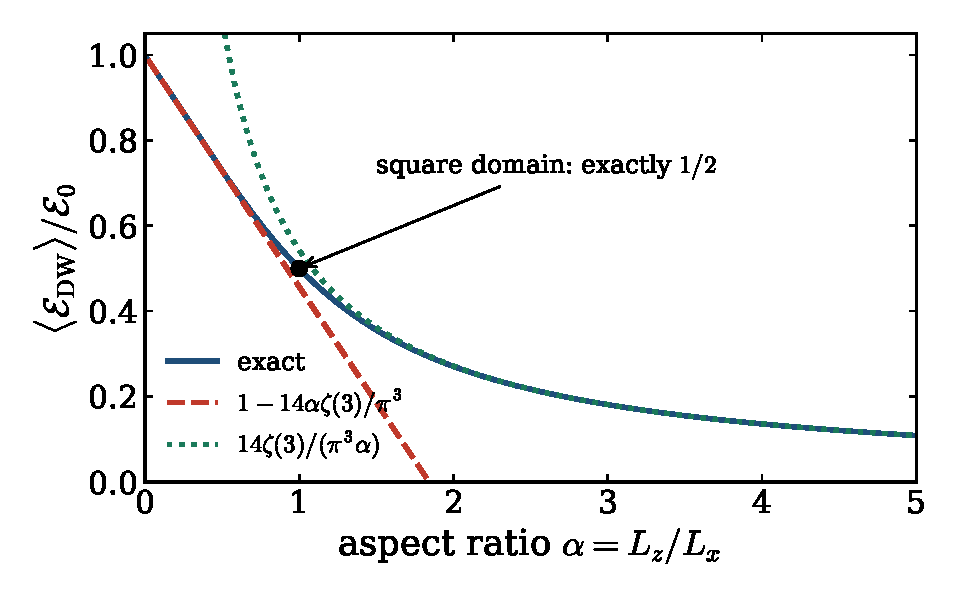
\includegraphics[width=0.5\textwidth]{figs/csl_dwenergy.pdf}
\end{frame}

\begin{frame}{Backup: towards quantum simulation of the CSL}
Discretise the same Hamiltonian on $N$ sites, $Q=2^{n_q}$ field values per site,
$\hat Z|k\rangle=\omega^k|k\rangle$, $\hat X|k\rangle=|k{+}1\rangle$:
\[
 \hat H=t\sum_n\hat\Pi_n^2+J\sum_{\langle nm\rangle}(1-\cos\Delta\varphi)
 +h\sum_n(1-\cos\varphi_n)-\kappa\sum_{\langle nm\rangle}\sin\Delta\varphi
\]
with $t=\frac{1}{2\fpi^2a}$, $J=\frac{\fpi^2}{a}$, $h=\fpi^2\mpi^2a$,
$\kappa=\fpi^2H=\frac{\mu B}{4\pi^2}$ ($a$-independent --- it is topological).
\vspace{1mm}
\begin{columns}[T,onlytextwidth]
\begin{column}{0.54\textwidth}
Exact for any $Q$:
$\cos\varphi\to\frac12(\hat Z+\hat Z^\dagger)$,
$\cos\Delta\varphi\to\frac12(\hat Z_{n+1}\hat Z_n^\dagger+\text{h.c.})$, and
\[
 \hat\Pi^2=\frac{Q^2+2}{12}\bm{1}
 +\sum_{m=1}^{Q-1}\frac{(-1)^m}{2\sin^2(\pi m/Q)}\hat X^m
\]
\end{column}
\begin{column}{0.46\textwidth}
\begin{alertblock}{A physics constraint on the encoding}
For $n_q=1$, $\Delta\varphi\in\{0,\pm\pi\}$ so $\sin\Delta\varphi\equiv0$: the
magnetic term \emph{drops out identically}.\\[1mm]
\alert{The CSL first exists at 2 qubits per site.}
\end{alertblock}
\end{column}
\end{columns}
\end{frame}

\begin{frame}{References}
\footnotesize
\begin{itemize}
  \item D.\,T.~Son, M.\,A.~Stephanov, \emph{Axial anomaly and magnetism of
        nuclear and quark matter}, PRD \textbf{77} (2008) 014021
        [arXiv:0710.1084].
  \item T.~Brauner, N.~Yamamoto, \emph{Chiral soliton lattice and charged pion
        condensation in strong magnetic fields}, JHEP \textbf{04} (2017) 132
        [arXiv:1609.05213].
  \item T.~Brauner, R.~Radhakrishnan, \emph{Chiral soliton lattice in
        inhomogeneous magnetic fields}, arXiv:2608.27319.
  \item D.\,T.~Son, A.\,R.~Zhitnitsky, PRD \textbf{70} (2004) 074018.
  \item T.~Brauner, H.~Kole\v{s}ov\'a, N.~Yamamoto, PLB \textbf{823} (2021)
        136767; T.~Brauner, H.~Kole\v{s}ov\'a, JHEP \textbf{07} (2023) 163.
  \item L.~Levkova, C.~DeTar, PRL \textbf{112} (2014) 012002
        (domain-wall magnetic fields on the lattice).
  \item T.~Kar, \emph{Finite volume correction to chiral soliton lattice in
        QCD}, MSc thesis, SVNIT Surat (2022).
  \item Y.~Togawa \emph{et al.}, PRL \textbf{108} (2012) 107202
        (CSL in chiral magnets).
\end{itemize}
\end{frame}

\end{document}
